
\documentclass{beamer}
\usetheme{Madrid}

\title{Building a GNU/Hurd Cluster}
\author{Brent Baccala}
\institute{\tt cosine@freesoft.org}
\date{January 17, 2018}

\setbeamertemplate{footline}{}
\beamertemplatenavigationsymbolsempty

\usepackage{color}
\usepackage{comment}
\usepackage{graphicx}

\usepackage{tabularx}

\usepackage{xstring}

\usepackage{tikz}
\usetikzlibrary{positioning, fit, backgrounds, arrows, patterns}

\begin{document}

\begin{frame}
\titlepage
\begin{block}{Abstract}
The GNU Hurd is a UNIX-like operating system based on Mach, an
operating system kernel developed at Carnegie Mellon University and
designed to support multi-node clusters, which have become ubiquitous
in high performance computing.  This talk will highlight current
trends in cluster computing, outline the design of Mach and Hurd, and
summarize the speaker's work to realize Hurd's potential as a
POSIX-compatible operating system that can leverage the power of an
entire cluster.
\end{block}
\end{frame}

\begin{frame}
\frametitle{Cisco 5108 Blade Server Chassis with eight B200 M2s}
\includegraphics[width=\textwidth]{ourcisco.jpg}
\end{frame}

\begin{frame}
\frametitle{Processor families in TOP500}
\includegraphics[width=\textwidth]{Processor_families_in_TOP500_supercomputers.png}
\end{frame}

\newcommand\topfh[7]{
#1 & #2 & #3 & #4 & #6 & #7 \\
& \multicolumn{4}{l}{\hskip 1cm #5} \\
\\
}

\begin{frame}
\frametitle{Top 10 positions of the TOP500 (November 2017)}
{\tiny
\begin{tabularx}{\textwidth}{lllllll}
\bf Rank
& \bf Name
& \bf Processor
& \bf Vendor
& \bf Cores
& \bf Operating system
\\
\\
\topfh{1}
{Sunway TaihuLight}
{SW26010}
{NRCPC}
{National Supercomputing Center in Wuxi, CHN}
{10,649,600}
{Linux (Raise)}

\topfh{2}
{Tianhe-2}
{Xeon E5–2692, Xeon Phi 31S1P}
{NUDT}
{National Supercomputing Center in Guangzhou, CHN}
{3,120,000}
{Linux (Kylin)}

\topfh{3}
{Piz Daint}
{Xeon E5-2690v3, Nvidia Tesla P100}
{Cray}
{Swiss National Supercomputing Centre, SWI}
{361,760}
{Linux (CLE)}

\topfh{4}
{Gyoukou}
{Xeon D-1571, PEZY-SC2}
{ExaScaler}
{Japan Agency for Marine-Earth Science and Technology, JAP}
{19,860,000}
{Linux (CentOS)}

\topfh{5}
{Titan}
{Opteron 6274, Nvidia Tesla K20X}
{Cray}
{Oak Ridge National Laboratory, USA}
{560,640}
{Linux (CLE, SLES based)}

\topfh{6}
{Sequoia}
{IBM A2}
{IBM}
{Lawrence Livermore National Laboratory, USA}
{1,572,864}
{Linux (RHEL and CNK)}

\topfh{7}
{Trinity}
{Xeon E5–2698v3, Xeon Phi}
{Cray}
{Los Alamos National Laboratory, USA}
{979,968}
{Linux (CLE)}

\topfh{8}
{Cori}
{Xeon Phi 7250}
{Cray}
{National Energy Research Scientific Computing Center, USA}
{622,336}
{Linux (CLE)}

\topfh{9}
{Oakforest-PACS}
{Xeon Phi 7250}
{Fujitsu}
{Kashiwa, Joint Center for Advanced High Performance Computing, JPN}
{556,104}
{Linux}

\topfh{10}
{K computer}
{SPARC64 VIIIfx}
{Fujitsu}
{Riken, Advanced Institute for Computational Science (AICS), JPN}
{705,024}
{Linux}

\end{tabularx}
Source: {\tt https://www.top500.org/}
}
\end{frame}

\begin{frame}[fragile]
\frametitle{Single System Image}
\begin{definition}
A single system image (SSI) cluster is a cluster of machines that appears to be one single system.

\hfill Wikipedia
\end{definition}
\begin{center}
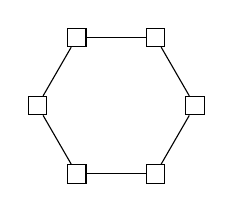
\begin{tikzpicture}
\node (a) [draw] at (0:1) {};
\node (b) [draw] at (60:1) {} edge (a);
\node (c) [draw] at (120:1) {} edge (b);
\node (d) [draw] at (180:1) {} edge (c);
\node (e) [draw] at (240:1) {} edge (d);
\node (f) [draw] at (300:1) {} edge (e) edge (a);
\end{tikzpicture}
\end{center}
\begin{semiverbatim}
\$ nproc
96
\$ free -h
              total        used        free
Mem:           768G         45G        723G
Swap:            0B          0B          0B

\end{semiverbatim}
\end{frame}

\begin{frame}
\frametitle{Single System Image}

\begin{itemize}
\item Key Features
\begin{itemize}
\item Cluster-wide login
\item Single Process Space
\item Process Migration
\item Single Root Filesystem
\item Redundant Filesystem
\item Single I/O Space - block devices
\item Single IPC Space
standard Linux inter-process communication mechanisms, shared memory, semaphores, SYSV message queues, pipes and Unix domain sockets.
\item Cluster-wide IP Addresses
\end{itemize}
\item Advantages
\begin{itemize}
\item familiar programming and management tools
\item ease of leveraging additional computing power
\end{itemize}
\item Disadvantages
\begin{itemize}
\item less fault isolation
\item node failure more difficult
\end{itemize}
\end{itemize}
\end{frame}

\begin{frame}
\frametitle{Cluster Computing - History}
\begin{itemize}
\item Beowulf
\item Hadoop
\item Cluster Linux
Kerrighed - Latest version is 3.0.0 which was released on 14 June 2010 and based on Linux kernel 2.6.30.
OpenSSI - last development release 2010; last stable release 2007
\end{itemize}
\end{frame}

\begin{frame}
\frametitle{Single System Image - History}
\begin{itemize}
\item VMS
\item SCALEMP
\item Cluster Linux
\end{itemize}
\end{frame}

\begin{frame}
\frametitle{GNU Hurd}
\begin{itemize}
\item History
\item Microkernels in general
\item CMU Mach
\end{itemize}
\end{frame}

\begin{frame}
\frametitle{CMU Mach}
\begin{itemize}
\item Tasks / Threads
\item Interprocess Communication
\item Memory Management
\end{itemize}
\end{frame}

\begin{frame}
\frametitle{Techniques to exploit parallelism}
\begin{itemize}
\item Instruction level parallelism
\begin{itemize}
\item Superscalar vector operations
\item Speculative execution
\end{itemize}
\item Thread level parallelism
\item Node level parallelism
\begin{itemize}
\item Clusters
\end{itemize}
\end{itemize}
\end{frame}

\begin{frame}[fragile]
\frametitle{Adding 512 64-bit integers - conventional x86-64 instrs}
\begin{semiverbatim}
\tiny
int a[512];
int b[512];
int c[512];

int main () \{
  for (int i=0; i<512; i++) \{
    a[i] = b[i] + c[i];
  \}
\}

gcc -O2 -o ex2 ex2.c

00000000004003e0 <main>:
4003e0:31 c0                xor    %eax,%eax
4003e2:66 0f 1f 44 00 00    nopw   0x0(%rax,%rax,1)
4003e8:8b 90 60 18 60 00    mov    0x601860(%rax),%edx
4003ee:03 90 60 10 60 00    add    0x601060(%rax),%edx
4003f4:48 83 c0 04          add    $0x4,%rax
4003f8:89 90 5c 20 60 00    mov    %edx,0x60205c(%rax)
4003fe:48 3d 00 08 00 00    cmp    $0x800,%rax
400404:75 e2                jne    4003e8 <main+0x8>
400406:31 c0                xor    %eax,%eax
400408:c3                   retq   

\end{semiverbatim}
\vskip 0pt plus 100fill
\end{frame}

\begin{frame}[fragile]
\frametitle{Adding 512 64-bit integers - SSE superscalar instructions}
\begin{semiverbatim}
\tiny
int a[512] __attribute__((aligned(0x10)));
int b[512] __attribute__((aligned(0x10)));
int c[512] __attribute__((aligned(0x10)));

int main () \{
  for (int i=0; i<512; i++) \{
    a[i] = b[i] + c[i];
  \}
\}

gcc -O3 -o ex2 ex2.c

00000000004003e0 <main>:
4003e0:31 c0                xor    %eax,%eax
4003e2:66 0f 1f 44 00 00    nopw   0x0(%rax,%rax,1)
4003e8:66 0f 6f 80 40 10 60 movdqa 0x601040(%rax),%xmm0
4003ef:00 
4003f0:48 83 c0 10          add    $0x10,%rax
4003f4:66 0f fe 80 30 18 60 paddd  0x601830(%rax),%xmm0
4003fb:00 
4003fc:0f 29 80 30 20 60 00 movaps %xmm0,0x602030(%rax)
400403:48 3d 00 08 00 00    cmp    $0x800,%rax
400409:75 dd                jne    4003e8 <main+0x8>
40040b:31 c0                xor    %eax,%eax
40040d:c3                   retq   

\end{semiverbatim}
\vskip 0pt plus 100fill
\end{frame}

\begin{frame}[fragile]
\frametitle{Adding 512 64-bit integers - AVX2 superscalar instructions}
\begin{semiverbatim}
\tiny
int a[512] __attribute__((aligned(0x20)));
int b[512] __attribute__((aligned(0x20)));
int c[512] __attribute__((aligned(0x20)));

int main () \{
  for (int i=0; i<512; i++) \{
    a[i] = b[i] + c[i];
  \}
\}

gcc -march=native -O3 -o ex2 ex2.c

00000000004003e0 <main>:
4003e0:31 c0                xor    %eax,%eax
4003e2:66 0f 1f 44 00 00    nopw   0x0(%rax,%rax,1)
4003e8:c5 fd 6f 80 60 10 60 vmovdqa 0x601060(%rax),%ymm0
4003ef:00 
4003f0:c5 fd fe 80 60 18 60 vpaddd 0x601860(%rax),%ymm0,%ymm0
4003f7:00 
4003f8:48 83 c0 20          add    $0x20,%rax
4003fc:c5 fd 7f 80 40 20 60 vmovdqa %ymm0,0x602040(%rax)
400403:00 
400404:48 3d 00 08 00 00    cmp    $0x800,%rax
40040a:75 dc                jne    4003e8 <main+0x8>
40040c:c5 f8 77             vzeroupper 
40040f:31 c0                xor    %eax,%eax
400411:c3                   retq   

\end{semiverbatim}
\vskip 0pt plus 100fill
\end{frame}

\begin{frame}[fragile]
\frametitle{Adding 512 64-bit integers - AVX512 superscalar instrs}
\begin{semiverbatim}
\tiny
int a[512] __attribute__((aligned(0x40)));
int b[512] __attribute__((aligned(0x40)));
int c[512] __attribute__((aligned(0x40)));

int main () \{
  for (int i=0; i<512; i++) \{
    a[i] = b[i] + c[i];
  \}
\}

gcc -mavx512vl -O3 -o ex2 ex2.c

00000000004003e0 <main>:
4003e0:31 c0                xor    %eax,%eax
4003e2:66 0f 1f 44 00 00    nopw   0x0(%rax,%rax,1)
4003e8:62 f1 fd 48 6f 80 80 vmovdqa64 0x601080(%rax),%zmm0
4003ef:10 60 00 
4003f2:48 83 c0 40          add    $0x40,%rax
4003f6:62 f1 7d 48 fe 80 40 vpaddd 0x601440(%rax),%zmm0,%zmm0
4003fd:14 60 00 
400400:62 f1 fd 48 7f 80 40 vmovdqa64 %zmm0,0x601840(%rax)
400407:18 60 00 
40040a:48 3d 00 08 00 00    cmp    $0x800,%rax
400410:75 d6                jne    4003e8 <main+0x8>
400412:31 c0                xor    %eax,%eax
400414:c3                   retq   

baccala@ideapad-S510p:~$ ./ex2
Illegal instruction (core dumped)
baccala@ideapad-S510p:~$ ./ex2

\end{semiverbatim}
\vskip 0pt plus 100fill
\end{frame}

\begin{frame}[fragile]
\frametitle{Pointer Aliasing}
\begin{semiverbatim}
\tiny
void operation (int * a, int * b, int * c)
\{
  for (int i=0; i<16; i++) \{
    c[i] = a[i] + b[i];
  \}
\}
\end{semiverbatim}
\pause
\begin{semiverbatim}
\tiny
int v[18] = \{1, 1\};

int main () \{
  operation(\&v[0], \&v[1], \&v[2]);

  for (int i=0; i<18; i++) \{
    printf("%d ", v[i]);
  \}
  printf("\\n");
\}
\end{semiverbatim}
What does this code do?
\pause
\begin{semiverbatim}
\tiny
baccala@blade6:~\$ ./ex4
1 1 2 3 5 8 13 21 34 55 89 144 233 377 610 987 1597 2584 
baccala@blade6:~\$
\end{semiverbatim}
\end{frame}


\begin{frame}[fragile]
\frametitle{Pointer Aliasing - The {\tt restrict} keyword}
\begin{semiverbatim}
\tiny
void operation (int * restrict a, int * restrict b, int * restrict c)
\{
  for (int i=0; i<16; i++) \{
    a[i] = b[i] + c[i];
  \}
\}


gcc -mavx512vl -O3 -c ex3.c

0000000000000000 <operation>:
   0:   62 f1 7e 48 6f 06       vmovdqu32 (%rsi),%zmm0
   6:   62 f1 7d 48 fe 02       vpaddd (%rdx),%zmm0,%zmm0
   c:   62 f1 7e 48 7f 07       vmovdqu32 %zmm0,(%rdi)
  12:   c3                      retq   

\end{semiverbatim}
\end{frame}

\begin{frame}
\frametitle{Intel Ivy Bridge Processor}
\includegraphics[width=\textwidth]{ivybridge.jpg}
\begin{center}
\huge
Notice the size of the graphics co-processor!
\end{center}
\end{frame}

\begin{comment}
\begin{frame}[fragile]
\begin{semiverbatim}
\tiny
import java.io.IOException;
import java.util.StringTokenizer;

import org.apache.hadoop.conf.Configuration;
import org.apache.hadoop.fs.Path;
import org.apache.hadoop.io.IntWritable;
import org.apache.hadoop.io.Text;
import org.apache.hadoop.mapreduce.Job;
import org.apache.hadoop.mapreduce.Mapper;
import org.apache.hadoop.mapreduce.Reducer;
import org.apache.hadoop.mapreduce.lib.input.FileInputFormat;
import org.apache.hadoop.mapreduce.lib.output.FileOutputFormat;

public class WordCount \{

  public static class TokenizerMapper
       extends Mapper<Object, Text, Text, IntWritable>\{

    private final static IntWritable one = new IntWritable(1);
    private Text word = new Text();

    public void map(Object key, Text value, Context context
                    ) throws IOException, InterruptedException \{
      StringTokenizer itr = new StringTokenizer(value.toString());
      while (itr.hasMoreTokens()) \{
        word.set(itr.nextToken());
        context.write(word, one);
      \}
    \}
  \}

  public static class IntSumReducer
       extends Reducer<Text,IntWritable,Text,IntWritable> \{
    private IntWritable result = new IntWritable();

    public void reduce(Text key, Iterable<IntWritable> values,
                       Context context
                       ) throws IOException, InterruptedException \{
      int sum = 0;
      for (IntWritable val : values) \{
        sum += val.get();
      \}
      result.set(sum);
      context.write(key, result);
    \}
  \}

  public static void main(String[] args) throws Exception \{
    Configuration conf = new Configuration();
    Job job = Job.getInstance(conf, ``word count'');
    job.setJarByClass(WordCount.class);
    job.setMapperClass(TokenizerMapper.class);
    job.setCombinerClass(IntSumReducer.class);
    job.setReducerClass(IntSumReducer.class);
    job.setOutputKeyClass(Text.class);
    job.setOutputValueClass(IntWritable.class);
    FileInputFormat.addInputPath(job, new Path(args[0]));
    FileOutputFormat.setOutputPath(job, new Path(args[1]));
    System.exit(job.waitForCompletion(true) ? 0 : 1);
  \}
\}
\end{semiverbatim}
\end{frame}
\end{comment}

\begin{frame}[fragile]
\frametitle{Hadoop MapReduce Tutorial - WordCount}
\begin{semiverbatim}
\tiny public class WordCount \{

  public static class TokenizerMapper
       extends Mapper<Object, Text, Text, IntWritable>\{

    private final static IntWritable one = new IntWritable(1);
    private Text word = new Text();

    public void map(Object key, Text value, Context context)
                     throws IOException, InterruptedException \{
      StringTokenizer itr = new StringTokenizer(value.toString());
      while (itr.hasMoreTokens()) \{
        word.set(itr.nextToken());
        context.write(word, one);
      \}
    \}
  \}

  public static class IntSumReducer
       extends Reducer<Text,IntWritable,Text,IntWritable> \{
    private IntWritable result = new IntWritable();

    public void reduce(Text key, Iterable<IntWritable> values, Context context)
                        throws IOException, InterruptedException \{
      int sum = 0;
      for (IntWritable val : values) \{
        sum += val.get();
      \}
      result.set(sum);
      context.write(key, result);
    \}
  \}
\}
\end{semiverbatim}
\end{frame}

% tikz commands to draw task boxes to illustrate Mach IPC concepts

\tikzstyle{task} = [draw, fill=blue!20, rounded corners]

\tikzstyle{message} = [draw, fill=red!20, text width=5em, text depth=3em, text centered,
  minimum width=5em, minimum height=2em, rounded corners]

% \task - takes four arguments
% 1. name of task
% 2. location of task box's center point
% 3. "r" or "l", indicating if a set of tick marks representing
%    ports should drawn on the left or right side of the task box
%    "u" to make the task unlabled
% 4. contents of the task box - other nodes
%
% The tick marks will be named "#1 Port #" for future reference

\newcommand\task[4]{
\matrix (#1) [task, inner xsep=0] at (#2) { \node {\IfSubStr{#3}{u}{}{#1}}; \\ #4

% print port tick marks in fill color if they are disabled, in order to make
% them expand out the dimensions of the task box yet remain invisible

\foreach \i in {-7,...,7}
{
\IfSubStr{#3}{l}{
  \draw[xshift=-5em, ultra thick] (0,0.2 * \i)  coordinate (#1 Port \i) -- (0.2,0.2 * \i);
}{
  \draw[xshift=-5em, ultra thick, color=blue!20] (0,0.2 * \i) -- (0.2,0.2 * \i);
}
\IfSubStr{#3}{r}{
  \draw[xshift=5em, ultra thick] (-0.2,0.2 * \i) -- (0,0.2 * \i) coordinate (#1 Port \i);
}{
  \draw[xshift=5em, ultra thick, color=blue!20] (-0.2,0.2 * \i) -- (0,0.2 * \i);
}
}

\\};
}

\begin{frame}
\frametitle{Ports - Mach's Interprocess Communication (IPC)}

\begin{center}

\begin{tikzpicture}[transform canvas={scale=0.4, yshift=10em, xshift=-15em}]

\task{Task 1 left}{0,0}{ru}{}
\task{Task 2 left}{0,-11 em}{ru}{}
\task{Task 3 left}{0,-22 em}{ru}{}
\task{Task 4 left}{0,-33 em}{ru}{}
\task{Task 1 right}{30 em,0}{lu}{}
\task{Task 2 right}{30 em,-11 em}{lu}{}
\task{Task 3 right}{30 em,-22 em}{lu}{}
\task{Task 4 right}{30 em,-33 em}{lu}{}

\draw [color=violet, thick, -triangle 90] (Task 1 left Port 5) -- (Task 1 right Port 5);
\draw [color=violet, thick] (Task 2 left Port 0) -- +(1,0) |- (Task 1 right Port 5);
\draw [color=violet, thick, -triangle 90] (Task 2 left Port 5) -- (Task 2 right Port 5);
\draw [color=violet, thick, triangle 90-] (Task 2 left Port -5) -- (Task 2 right Port -5);

\filldraw[fill=white] (Task 1 right Port 5) ++(-4,-0.5) rectangle +(1.8,1);
\filldraw[fill=white, pattern=vertical lines] (Task 1 right Port 5) ++(-4,-0.5) rectangle +(1.8,1);

\filldraw[fill=white] (Task 2 right Port 5) ++(-4,-0.5) rectangle +(1.8,1);
\filldraw[fill=white, pattern=vertical lines] (Task 2 right Port 5) ++(-4,-0.5) rectangle +(1.8,1);

\filldraw[fill=white] (Task 2 right Port -5) ++(-4,-0.5) rectangle +(1.8,1);
\filldraw[fill=white, pattern=vertical lines] (Task 2 right Port -5) ++(-4,-0.5) rectangle +(1.8,1);

\end{tikzpicture}
\end{center}

\end{frame}

\begin{frame}
\frametitle{Mach IPC}

\begin{center}

\begin{tikzpicture}

\task{Task 1}{0,0}{r}{
\node (message1) [message] {Message 1};
}
\task{Task 2}{15 em,0}{l}{
\node (message2) [message] at (1 em, 1 em) {Message 1};
\node (message2a) [message] at (1.9 em, -1 em) {Message 2};
}
\task{Task 3}{0,-11 em}{r}{
\node (message3) [message] {Message 2};
}


\draw [color=violet, thick, ->] (node cs:name=message1,angle=20) -- +(.3,0) |- (Task 1 Port 5) node [midway, anchor=south, color=black] {27} -- (Task 2 Port 5)
    -- +(.5,0) node [at end, anchor=south, color=black] {52} |- (node cs:name=message2, angle=160);

\draw [color=violet, thick, ->] (node cs:name=message3,angle=0) -- +(.3,0) |- (Task 3 Port 0) node [midway, anchor=south, color=black] {18} -- +(1,0) |- (Task 2 Port 5)
    -- +(.5,0) |- (node cs:name=message2a, angle=160);

\end{tikzpicture}
\end{center}

\end{frame}

\begin{frame}

\frametitle{Send Rights}

\begin{center}

\begin{tikzpicture}

\task{Task 1}{0,0}{r}{
% print two sendright nodes, one to fill the message1 box to the correct size,
% and another one to actually draw it, since message1 will overwrite the
% first sendright
\node (sendright) [draw, fill=orange] {Send 41};
\node (message1) [fit=(sendright), message] {Message 1};
\node (sendright) [draw, fill=orange] {Send 41};

\node (message3) at (0, -7em) [message] {Message 2};
}

\task{Task 2}{15 em,0}{l}{
\node (sendright2) [draw, fill=orange] {Send 9};
\node (message2) [fit=(sendright2), message] {Message 1};
\node (sendright2) [draw, fill=orange] {Send 9};

\node (message4) at (0, -7em) [message] {Message 2};
}


\draw [color=violet, thick, ->] (node cs:name=message1,angle=20) -- +(.3,0) |- (Task 1 Port 5) node [midway, anchor=south, color=black] {27} -- (Task 2 Port 5)
    -- +(.5,0) node [at end, anchor=south, color=black] {52} |- (node cs:name=message2, angle=160);

\draw [color=violet, thick, <-] (node cs:name=message3,angle=20) -- +(.3,0) |- (Task 1 Port -5) node [midway, anchor=south, color=black] {41} -- (Task 2 Port -5)
    -- +(.5,0) node [near end, anchor=south, color=black] {9} |- (node cs:name=message4, angle=160);

\end{tikzpicture}
\end{center}

\end{frame}




\begin{frame}

\frametitle{Send Rights}

\begin{center}

\begin{tikzpicture}

\task{Task 1}{0,0}{r}{
% print two sendright nodes, one to fill the message1 box to the correct size,
% and another one to actually draw it, since message1 will overwrite the
% first sendright
\node (sendright) [draw, fill=orange] {Send 41};
\node (message1) [fit=(sendright), message] {Message 1};
\node (sendright) [draw, fill=orange] {Send 41};
}
\task{Task 2}{15 em,0}{l}{
\node (sendright2) [draw, fill=orange] {Send 9};
\node (message2) [fit=(sendright2), message] {Message 1};
\node (sendright2) [draw, fill=orange] {Send 9};
%\node (message2) [message] {Message 1};
% \node (message2a) [message] at (1 em, -2 em) {Message 2};
}
\task{Task 1 }{0,-11 em}{r}{
\node (message3) [message] {Message 2};
}
\task{Task 2 }{15 em,-11 em}{l}{
\node (message4) [message] {Message 2};
}


\draw [color=violet, thick, ->] (node cs:name=message1,angle=20) -- +(.3,0) |- (Task 1 Port 5) node [midway, anchor=south, color=black] {27} -- (Task 2 Port 5)
    -- +(.5,0) node [at end, anchor=south, color=black] {52} |- (node cs:name=message2, angle=160);

%\draw [color=violet, thick, ->] (node cs:name=message3,angle=0) -- +(.3,0) |- (Task 3 Port 0) node [midway, anchor=south, color=black] {18} -- +(1,0) |- (Task 2 Port 3)
%    -- +(.3,0) |- (node cs:name=message2a, angle=160);

\end{tikzpicture}
\end{center}

\end{frame}

\begin{frame}
\frametitle{Right Transfers}
\end{frame}

\begin{frame}
\frametitle{Memory Transfers}
\end{frame}

\begin{frame}
\frametitle{Hurd Filesystem}
\end{frame}

\begin{frame}
\frametitle{Example: Basic File I/O}
\end{frame}

\begin{frame}
\frametitle{Mach Memory Management}
\end{frame}

\begin{frame}
\frametitle{Example: Shared Libraries}
\end{frame}

\begin{frame}[fragile]
\frametitle{Pseudocode: {\tt memory\_object\_data\_request}}
\begin{semiverbatim}
\tiny
memory_object_data_request: (kernel requesting a single page)

  if TERMINATING flag set, return
  if this client is on NEXTERROR list and WRITE ACCESS WAS REQUESTED, send a m_o_data_error message,
        move NEXTERROR to ERROR, remove the NEXTERROR list entry, and return
  if the page is PAGINGOUT:
    if WAITLIST is empty and ACCESSLIST is not, send lock request (internal flush) to ACCESSLIST client
       ASSERT: there should only be one WRITE client on ACCESSLIST
               (the client that returned the data we're paging out)
    add requesting client to WAITLIST and return
  if this client is already on ACCESSLIST, it flushed and is trying to re-aquire access,
     so check to see if WAITLIST is empty
     if so, remove client from ACCESSLIST and proceed (kernel flushed without being asked)
     if not, we're flushing, so add client to WAITLIST, run internal_lock_completed on this page, and return
  if WAITLIST is not empty, add requesting client to WAITLIST and return
  if another client has WRITE access (WAITLIST is empty), add requesting client to WAITLIST,
     send lock request (internal flush variant) and return
  if WRITE access is requested and ACCESSLIST is not empty (other clients have access),
     add requesting client to WAITLIST (it's empty),
     send lock requests (internal flush variant) and return
     (we could give out the page with READ access and wait for a unlock request, but I think not)
  else
     (ACCESSLIST is empty or READ access is requested and only READ clients are on ACCESSLIST)
     if page is flagged INVALID, send m_o_data_error to this client and return
     add this client to WAITLIST (it's empty)
     unlock pager
     read the page with pager_read_page()
     relock pager
     if pager_read_page() returned an error, mark page with ERROR and call send_error_to_WAITLIST
     if no error, service_waitlist(deallocate=true) (read/write status supplied by filesystem), clear ERROR
\end{semiverbatim}
\end{frame}

% https://events.ccc.de/congress/2007/Fahrplan/attachments/986_inside_the_mac_osx_kernel.pdf

% Mac OS X Internals: A Systems Approach

\end{document}
